\documentclass[11pt]{article}
\usepackage{graphicx} % Required for inserting images
\usepackage[top=2.5cm, bottom=2.5cm, left=2cm, right=2cm]{geometry}
\usepackage[T1]{fontenc}
\usepackage{wrapfig}
\usepackage{hyperref}
\usepackage[utf8]{inputenc}
\usepackage{multirow}
\usepackage{subcaption}
\usepackage{booktabs}
\usepackage{bookmark}
\usepackage{graphicx}
\usepackage{setspace}
\usepackage{listings}
\usepackage{xcolor}  % Opcional, per colors
\lstset{
  language=Python,
  basicstyle=\ttfamily\small,
  keywordstyle=\color{blue},
  commentstyle=\color{gray},
  stringstyle=\color{green!50!black},
  showstringspaces=false,
  numbers=left,
  numberstyle=\tiny\color{gray},
  frame=single,
  breaklines=true,
  captionpos=b,
  tabsize=4
}

\setlength{\parindent}{0in}
\usepackage{physics}
\usepackage{tikz}
\usepackage{tikz-3dplot}
\usepackage[outline]{contour} % glow around text
\usepackage{xcolor}
\usepackage{float}
\usepackage{makeidx}
\usepackage{fancyhdr}
\usepackage{pgfplots}
\usepackage{amsmath}
\pgfplotsset{compat=1.18}
\usepackage{caption}
\usepackage[english,catalan]{babel}
\setlength{\parskip}{11pt}
\usepackage{xcolor}
\usepackage{listings}
\usepackage{marginnote}
\usepackage{siunitx}
\usepackage{framed}
\usepackage{ulem}

\begin{document}
\tableofcontents
\newpage
\vspace{10em}

{\huge \textbf{Pràctica 1}}  % Títol petit en negreta

\vspace{0.5em}  % Espai vertical

{\Huge \textbf{Representació de camps}}  % Títol gran

\vspace{2em}  % Espai abans del contingut

%\title{\Huge\bfseries Pràctica 1 \\ Feixos de raigs catòdics \\ [2ex] \Large}

\begin{abstract}
    En aquesta pràctica estudiem les línies equipotencials i de camp de tres distribucions de conductors en un medi dielèctric assumint simetria en l'eix vertical. Un condensador plano-paral·lel, dos fils infinits i una geometria escollida entre els membres del grup que replica la disposició d'un experiment de difracció. Els resultats obtinguts són corroborats per simulacions computacionals i comparats amb els resultats del cas ideal dels què en difereix substancialment. També s'obté experimentalment la capacitat del condensador i es conclou que no difereix significativament del càlcul ideal.
\end{abstract}


\section{Introducció teòrica}\label{sec: intro}
En aquesta pràctica trobem experimentalment les línies equipotencials i de camp de tres distribucions de conductors en un material dielèctric de difícil o inexistent solució analítica, així com alguna propietat associada. La primera distribució estudiada és un condensador de plaques plano-paral·leles d'altura infinita i llargada finita, del qual també en calculem la capacitat; la segona són dos fils infinits paral·lels a diferents potencials; i per últim, estudiem una placa amb una escletxa davant d'un fil infinit a diferents potencials.

Per estudiar aquestes distribucions de conductors dins un medi dielèctric usem la dualitat que existeix entre el camp de corrents, $\vec{J}$, i el camp de desplaçament elèctric, $\vec{D}$. Com podem veure a les Eqs. (\ref{eq: J_D}) aquests dos camps tenen les mateixes equacions i, per tant, si repliquem les condicions de contorn d'un sistema en medi dielèctric en un sistema en medi conductor conductor, obtindrem les mateixes solucions per les corrents que obtindreim en el sistema dielèctirc pel camp de desplaçament.
\begin{equation}
    \begin{array}{lll}
    \vec{\nabla} \times \vec{J}=0 & \vec{J}=\sigma \vec{E} & \vec{\nabla} \cdot \vec{J}=0 \\
    \vec{\nabla} \times \vec{D}=0 & \vec{D}=\epsilon \vec{E} & \vec{\nabla} \cdot \vec{D}=0
    \end{array}
    \label{eq: J_D}
\end{equation}
Considerant que el medi dielèctric és lineal, isòtrop i homogeni (l.i.h), com veiem a les Eqs. (\ref{eq: J_D}), a través del camp de desplaçament i la permitivitat del medi dielèctric podem obtenir fàcilment la solució del camp elèctric i conseqüentment del potencial. A més, com que en aquest cas $\varepsilon$ i $g$ són escalars, el potencial complirà l'equació de Laplace
\begin{equation}
    \laplacian{\phi}=0.
\end{equation}
Així, usant un paper de carbó de conductivitat $g$ (que equival al medi dielèctric de permitivitat $\varepsilon$) i dibuixant-hi amb tinta conductora el sistema de conductors podem fer mesures del potencial que generaran els corrents i relacionar-lo amb el potencial elèctric de la mateixa distribució de conductors en un medi dielèctric.
Concretament, en aquesta pràctica els objectius que ens proposem són:
\begin{list}{$\ast$}{\leftmargin=1em}
    \item Determinar les línies equipotencials i de camp elèctric experimentals de
        \begin{enumerate}{\leftmargin=1em}
            \item  Un condensador de plaques plano-paral·leles d'alçada infinita però llargada finita.
            \item  Dos fils infinits paral·lels a diferents potencials.
            \item  Una placa amb una escletxa paral·lela a un fil infinit a diferents potencials.
        \end{enumerate}  
        i comparar-les amb els resultats simulats i els càlculs tèorics del cas ideal.
    \item Determinar la capacitat per unitat de longitud del condensador.
    \item (extra) Estimar la permetivitat relativa del medi dielèctric de l'experiment.
\end{list}

Pel que fa al càlcul experimental de la capacitat del condensador, anomenant $l$ a la llargada de les plaques (cap a la direcció $Y$), $L$ una altura arbitrària (cap a la direcció $Z$) i $d$ la distància de separació entre les plaques, podem procedir de la següent manera.
A partir de dues línies equipotencials que tanquin una de les plaques del condensador podem calcular la càrrega per unitat de longitud.
\begin{equation}
    \frac{Q}{L} = \frac{1}{L}\oint\vec{D}\vec{ds}=\varepsilon\oint Edl\approx \varepsilon \sum_i E_i \, \Delta l_i \approx \varepsilon \sum_i \frac{\Delta \phi_i \, \Delta l_i}{\Delta r_i}
    \label{eq: Q}
\end{equation}
On $\frac{Q }{L }$ és la càrrega per unitat de longitud del condensador, $\varepsilon$ la peritivitat del medi dielèctric, $\Delta \phi_i$ la diferència de potencial entre les línies equipotencials, $\Delta l_i$ un petit increment de distància sobre la línia equipotencial interior i $\Delta r_i$ la distància en aquest punt entre la línia equipotencial interior i l'exterior.
Aleshores, podem calcular la capacitat per unitat de longitud si sabem el potencial aplicat entre les plaques, $\Delta V$.
\begin{equation}
    \frac{C}{L}=\frac{Q/L}{\Delta V}
    \label{eq: C}
\end{equation}

Per altra banda, per obtenir la capacitat ideal d'un condensador de plaques plano-paral·lels com el que tenim a l'experiment calculem la diferència de potencial entre les plaques,
\begin{equation}
    |\Delta\phi|=\int_{0}^{d} \vec{E}\vec{dl}= Ed,
\end{equation}
i com que assumim que el camp és uniforme i de valor $\frac{\sigma}{\varepsilon}$\footnote{És molt fàcil obtenir aquest resultat sumant el camp de dos plans infinits de càrrega oposada que s'obté amb la llei de Gauss} podem obtenir la capacitat per unitat de longitud de la següent manera:
\begin{equation}
    \Delta\phi=Ed=\frac{\sigma d}{\varepsilon}
    =Q\frac{d}{lL\varepsilon}=\frac{Q}{C}\implies (\frac{C}{L})_t=\frac{l}{d}\varepsilon
    \label{eq: c_t}
\end{equation}

\section{Mètode experimental}\label{sec: metode}
Per dur a terme l'experiment hem dibuixat les tres configuracions esmentades anteriorment sobre uns rectangles de paper de carbó (de $28cm\cross20cm$) amb tinta conductora. Així doncs, hem traduït els nostres sistemes de tres dimensions (però amb simetria en un eix) a sistemes de dues dimensions dibuixant sobre el paper la secció dels conductors cap a la direcció $Z$. Per exemple, el condensador s'ha convertit en dues línies paral·leles o els dos fils infinits en dos punts. A l'Annex \ref{fotos} hi ha imatges de les tres configuracions que hem muntat al laboratori. Tot seguit, quan la tinta era seca, hem connectat el sistema a una font de corrent amb una diferència de potencial de $15 V$. En aquest punt és molt important comprovar que el conductor està ben dibuixat mirant si tots els punts tenen el mateix potencial. Finalment, amb un voltímetre hem anat marcant punts amb el mateix potencial per poder dibuixar les línies equipotencials.

En el cas del condensador és important que tingui les dimensions adequades. Ha de ser prou petit per obtenir línies tancades i que $\frac{d}{l}$ sigui prou petit perquè aquestes siguin paral·leles a la zona central del condensador. Unes bones mides per la dimensió del nostre paper són: $d=3cm$ i $l=8cm$.
Pel que fa al sistema de fils infinits, que sobre el paper representem com dos punts, és important que aquests siguin prou grans perquè les forquilles amb què els connectem a la font de corrent hi càpiguen i no generin interferències.

Per obtenir les dades necessàries pel càlcul de la capacitat del condensador, primerament hem dibuixat dues línies equipotencials tancades al voltant d'una de les plaques. Després hem dividit la línia interna en 20 segments i hem anat mesurant la llargada de cada segment ($\Delta l_i$), conjuntament amb la distància del segment a la línia equipotencial externa ($\Delta r_i$) i la diferència de potencial entre les dues línies ($\Delta \phi_i$).

Per representar els punts experimentals els hem digitalitzat amb el programa web WebPlotDigitizer\copyright\footnote{Enllaç a l'aplicació web: \url{https://automeris.io/wpd/}}. Així, també hem pogut dibuixar el camp elèctric calculant la direcció perpendicular a la recta entre dos punts experimentals adjacents amb un programa de Python.

Finalment, hem fet una simulació em Python per calcular computacionalment les línies equipotencials i de camp de les tres configuracions de conductors.\footnote{\label{nota: codis}Tots els codis es troben a l'Annex \ref{sec: python}}

\section{Resultats i discussió}\label{sec: resultats}
En aquesta secció presentem i comparem els resultats obtinguts tant experimentalment com computacionalment. Mostrem les línies de camp i les línies equipotencials de les tres distribucions de càrrega així com el resultat experimental de la capacitat d'una d'elles. Per fer les simulacions hem solucionat l'equació de Laplace amb el mètode de Jacobi\footnotemark[3]. Cal destacar que les simulacions les hem fet al buit, ja que no coneixem el valor de la permetivitat del dielèctric. A més, s'ha considerat que els elèctrodes són conductors ideals i constitueixen les úniques fonts del camp.

\subsection{Condensador de plaques plano-paral·leles}\label{sec: cond}
La primera distribució de càrrega que estudiarem és un condensador de plaques plano-paral·leles centrat a l'orígen. Les plaques són paral·leles al pla $YZ$, finites en la direcció $Y$ i molt llargues o infinies en la direcció $Z$.
En les Figs. (\ref{fig: cond_pot}) i (\ref{fig: cond_e}) podem veure representades les línies de camp elèctric i les línies equipotencials obtingudes tant experimentalment com en la simulació.   
\begin{figure}[h]
    \centering
    \begin{subfigure}{0.495\textwidth}
        \centering
        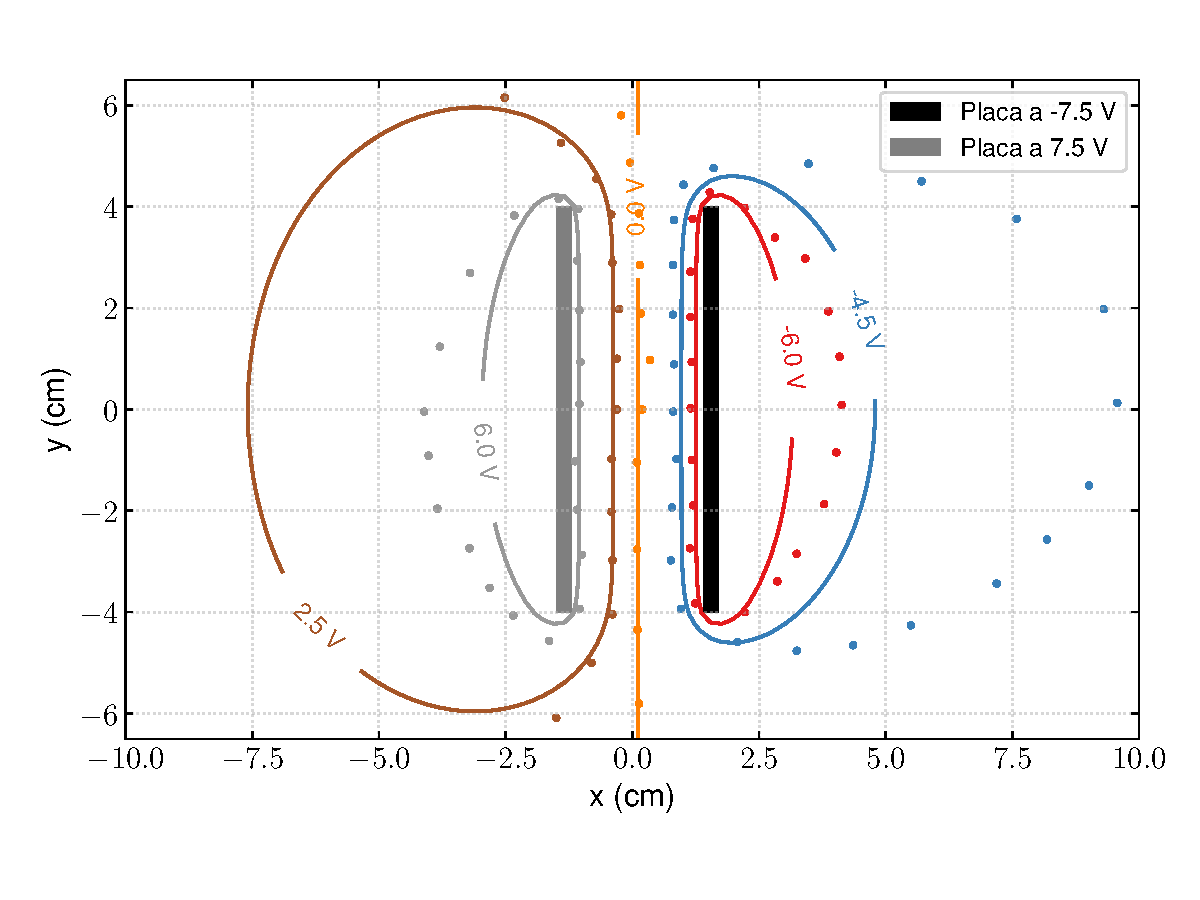
\includegraphics[width=\textwidth]{cond_combi_def.pdf}
        \caption{Línies equipotencials d'un condensador plano-paral·lel. Punts experimentals i línies de la simulació.}
        \label{fig: cond_pot}
    \end{subfigure}
    \begin{subfigure}{0.495\textwidth} 
        \centering
        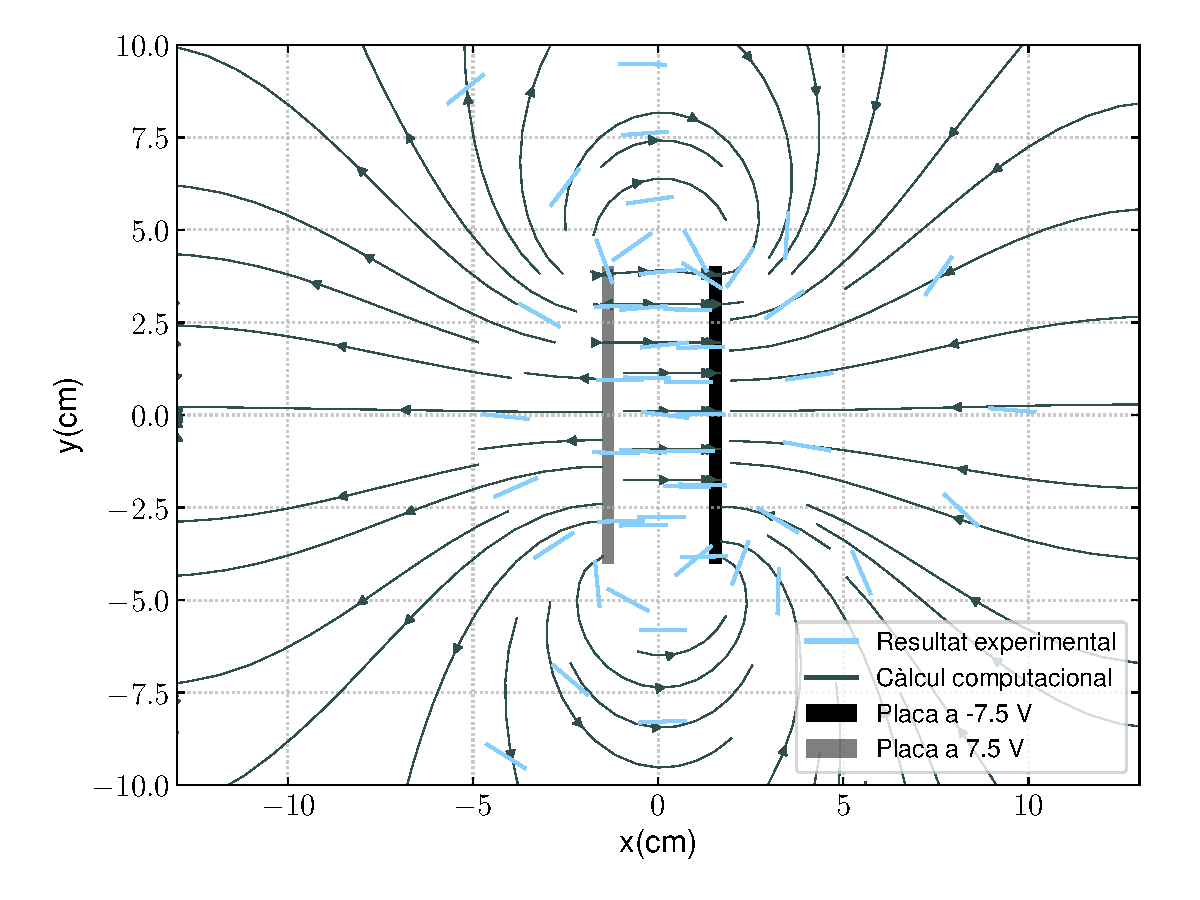
\includegraphics[width=\textwidth]{cond_camp.pdf}
        \caption{Línies de camp elèctric d'un condensador plano-paral·lel. Segments experimentals i línies de la simulació.}
        \label{fig: cond_e}
    \end{subfigure}
\end{figure}

A la Fig. (\ref{fig: cond_pot}) s'observa com a la regió central del condensador les línies equipotencials són paral·leles a les plaques, com prediu la teoria. En canvi, a prop de les vores, les línies es corben fins que s'acaben tancant a causa de la disminució de la component $Y$ del camp elèctric. Aquest resultat difereix del cas ideal, (condensador de plaques infinites) en el que les línies equipotencials mai es tanquen. Tanmateix, veiem que coinsideix amb la simulació, on les línies també es tanquen tot i que ho fan més a prop. Aquesta discrepància entre la simulació i l'experiment principalment és a causa de que la simulació està feta al buit i no té en compte la permetivitat relativa del medi. Això genera que el camp simulat sigui més intens i per tant, les línies equipotensials es tanquin més a prop de l'elèctrode. També hi ha altres efectes com les irregularitats dels elèctrodes, la connexió entre la font i els elèctrodes o la discontinuïtat del camp elèctric als límits del paper que no hem tingut en compte a la simulació i poden contribuir a la diferència dels resultats.

Pel que fa a la Fig. (\ref{fig: cond_e}) veiem com les línies de camp van des de la placa positiva a la negativa (com era d'esperar) i tenen major densitat a prop d'aquestes, indicant que el camp és més intens. Com en el cas del potencial, les línies segueixen un comportament semblant al ideal a la part central i, en canvi, a prop de les vores es desvien a causa dels efectes de vorada. Similarment, els segments experimentals, que representen la direcció del camp, també segueixen la tendència del càlcul computacional tot i que les línies experimentals tendeixen a tancar-se més sobre els elèctrodes. Aquestes diferències s'expliquen igual que les discutides anteriorment.

Per calcular la capacitat del condensador, primer hem calculat la càrrega per unitat de superfície del condensador en funció de $\varepsilon$, a partir de l'Eq. (\ref{eq: Q}). Tot seguit, amb l'Eq (\ref{eq: C}) hem calculat la capacitat per unitat de longitud del condensador (les dades necessàries per fer els càlculs es poden trobar a la Taula \ref{tab:mesures} de l'annex com també les Eqs. (\ref{eq: ins_q}), (\ref{eq: ins_c}) i (\ref{eq: ins_ct}) pel càlcul d'incerteses).

\[
\frac{Q}{L} = \varepsilon  (37{,}65 \pm 9{,}48)\, \mathrm{C/m} \implies
\boxed{ \frac{C}{L} = \varepsilon  (2{,}51 \pm 0{,}63)\, \mathrm{F/m} }
\]    

Aquest resultat el podem comparar amb el resultat tèoric de la capacitat d'un condensador ideal amb les mateixes dimensions. Usant l'Eq. (\ref{eq: c_t}) obtenim $(\frac{C}{L})_t =(2,667 \pm 0,095)\, \mathrm{F/m}$ que és compatible amb el resultat experimental del nostre condensador no ideal.

\subsection{Fils infinits}\label{sec: fils}
La segona configuració estudiada són dos fils infinits paral·lels amb càrrega oposada. Conseqüentment, en aquest cas, la simulació representa el cas ideal.
\begin{figure}[h]
    \centering
    \begin{subfigure}{0.495\textwidth}
        \centering
        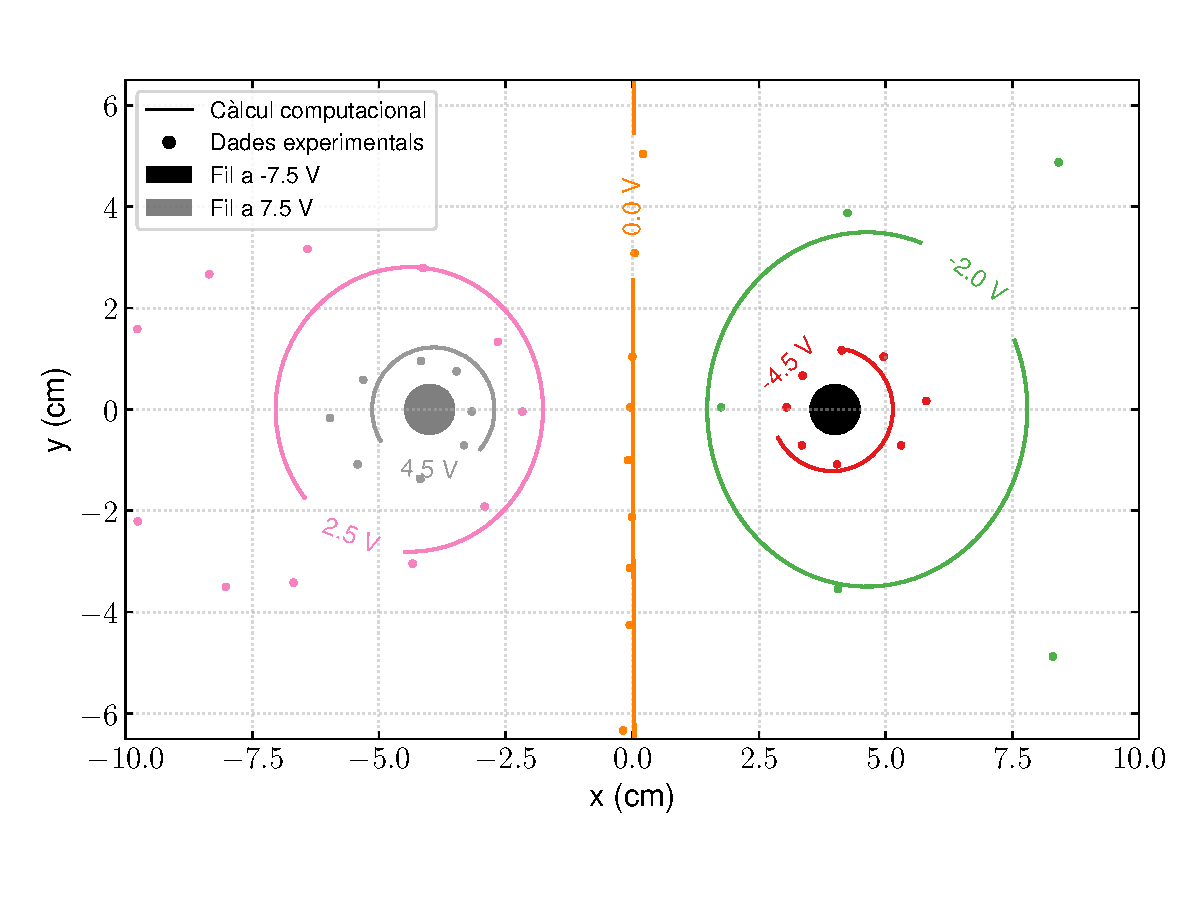
\includegraphics[width=\textwidth]{fils_combi.pdf}
        \caption{Línies equipotencials de dos fils infinits paral·lels i a potencials oposats.}
        \label{fig: fils_pot}
    \end{subfigure}
    \begin{subfigure}{0.495\textwidth} 
        \centering
        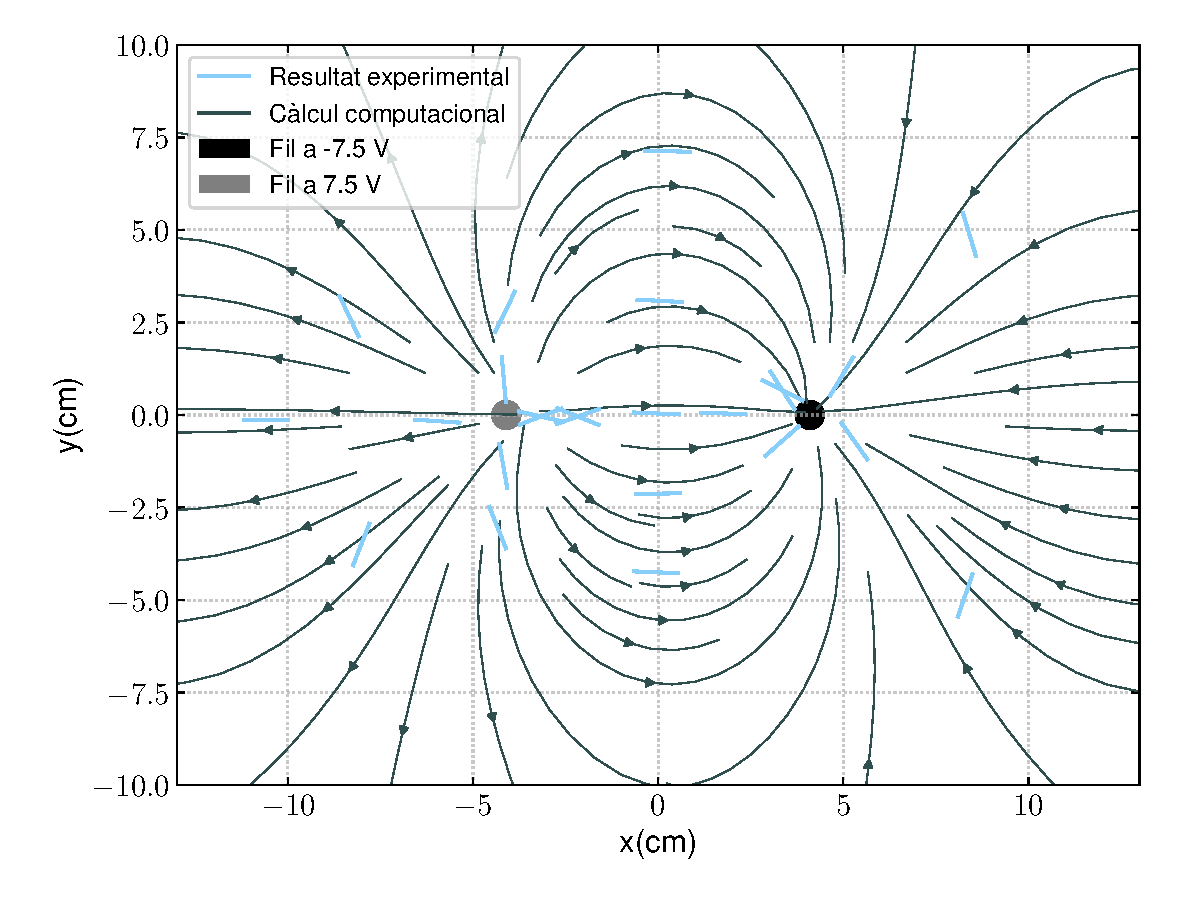
\includegraphics[width=\textwidth]{fils_camp.pdf}
        \caption{Línies de camp elèctric de dos fils infinits paral·lels i a potencials oposats. Segments experimentals i línies de la simulació.}
        \label{fig: fils_camp}
    \end{subfigure}
\end{figure}


A la Fig. (\ref{fig: fils_pot}), si ens fixem en les línies equipotencials experimentals veiem que es tanquen en el·lipses al voltant dels fils i presenten una assímptota just entre els dos elèctrodes. Aquesta és la tendència dictada per la simulació tot i que en la simulació les línies es tanquen en circumferències. Aquesta diferència pot ser deguda a diversos factors. En primer lloc, el nostre muntatge experimental és una aproximació en dues dimensions del sistema en tres dimensions que intentem replicar. En segon lloc, el nostre sistema té una discontinuïtat del camp elèctric als límits del paper (rectangular) que no hem introduït a la simulació. A més, a la simulació tampoc hem tingut en compte que el medi és dielèctric amb permitivitat diferent a $\varepsilon_0$. Per últim, pot haver altres contribuicions al camp que no hem tingut en compte com la unió entre els elèctrodes i la font de corrent o un camp extern present al laboratori.

Per altra banda, el camp elèctric  experimental mostrat a la Fig. (\ref{fig: fils_camp}) també segueix la tendència de la simulació tot i que les línies de camp que surten del fil a $7.5$ V tenen més tendència a tancar-se cap al fil a $-7.5$ V. Això pot ser degut a que hi ha diversos efectes que no hem tingut en compte a la simulació com hem explicat en el cas del potencial. 

\subsection{Placa amb escletxa i fil infinit}\label{sec:lliure}
La tercera configuració estudiada és un fil infinit enfront una placa infinita en l'eix $Z$ amb una escletxa al llarg de la placa i al davant del fil. A més, existeix una diferència de potencial entre el fil i les dues parts de la placa, què sí que estan al mateix potencial. Aquesta, és una disposició similar a la d'un experiment de difracció si tractem el fil com un "emissor" de línies equipotencials i les plaques amb l'escletxa com l'objecte que les difracta. Per tant, la motivació per estudiar aquesta configuració prové de voler veure si amb les línies de potencial passa algun fenomen similar a la difracció d'ones\footnote{Més informació sobre la difració d'ones a \url{https://en.wikipedia.org/wiki/Diffraction}}.

\begin{figure}[h]
    \centering
    \begin{subfigure}{0.495\textwidth}
        \centering
        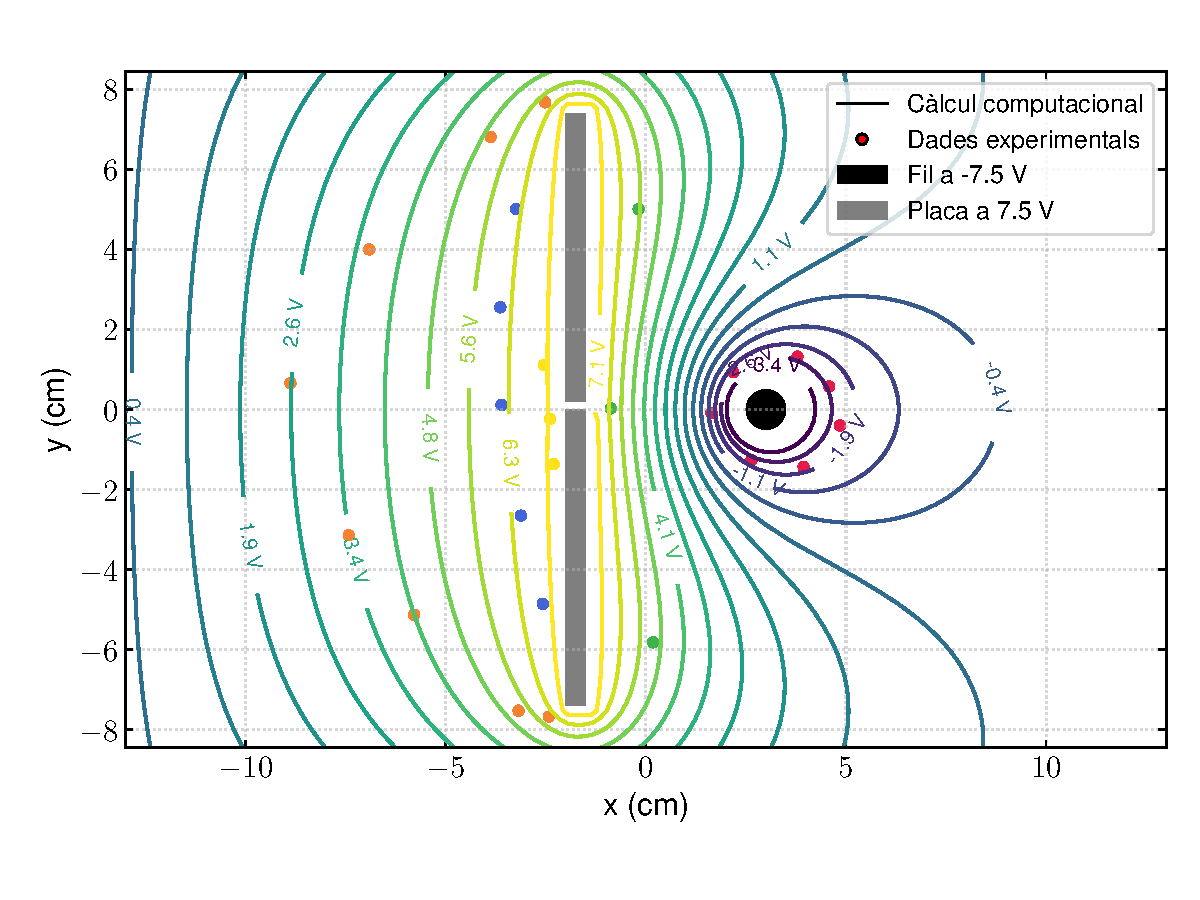
\includegraphics[width=\textwidth]{lliure_combi_e_colors.pdf}
        \caption{Línies equipotencials d'una placa infinita AMB escletxa davant d'un fil infinit. Punts experimentals de color diferent per cada valor de potencial.}
        \label{fig: lliure_pot_e}
    \end{subfigure}
    \begin{subfigure}{0.495\textwidth} 
        \centering
        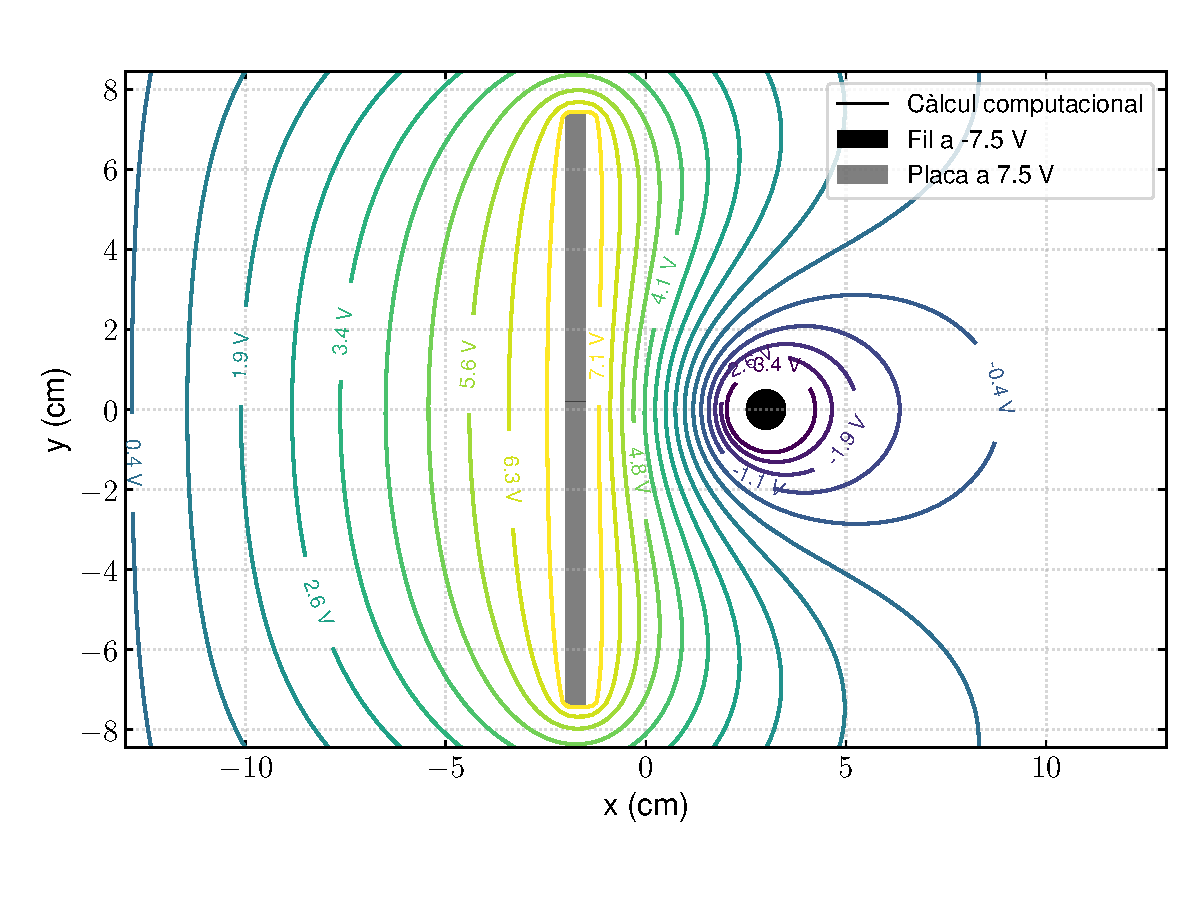
\includegraphics[width=\textwidth]{lliure_combi_0.pdf}
        \caption{Línies equipotencials d'una placa infinita SENSE escletxa davant d'un fil infinit.}
        \label{fig: lliure_pot_0}
    \end{subfigure}
\end{figure}
Si ens fixem en les línies equipotencials experimentals de la Fig. (\ref{fig: lliure_pot_e}) veiem que es comporten de la següent manera: el radi de corvatura de les línies equipotencials va augmentant a mesura que ens allunyem de l'"emissor" (fil) i ens apropem a l'escletxa, tal com ho faria el front d'una ona. A l'altra banda de l'escletxa, el radi de corvatura disminueix respecte l'observat abans de l'escletxa de tal forma que és com si l'escletxa fos un segon emissor. Per tant, amb aquesta informació sembla que hi hagi hagut un fenòment de difracció degut a l'escletxa.
No obstant això, si ens fixem en les línies equipotencials simulades veiem clarament que el motiu de la forma de les línies equipotencials no té res a veure amb l'escletxa. El veritable fet que explica les línies equipotencials mostrades és la superposició del potencial elèctric generat pel fil i la placa (que ja en coneixem la forma gràcies a les configuracions anteriors). De fet, com podem veure a la Fig. (\ref{fig: lliure_pot_0})l'existència de l'escletxa quasi bé no afecta a la forma de les línies equipotencials, ja que és molt petita en comparació amb les dimencions del fil i de la placa. Per tant, la difracció no serveix per explicar les observacions experimentals, tot i que, experimentalment, en un principi ho pugui semblar. Aquest resultat, era d'esperar ja que el potencial d'un sistema electroestàtic, per començar, no depen del temps i, per tant, no pot tenir propietats ondulatòries.
\begin{figure}
    \centering
    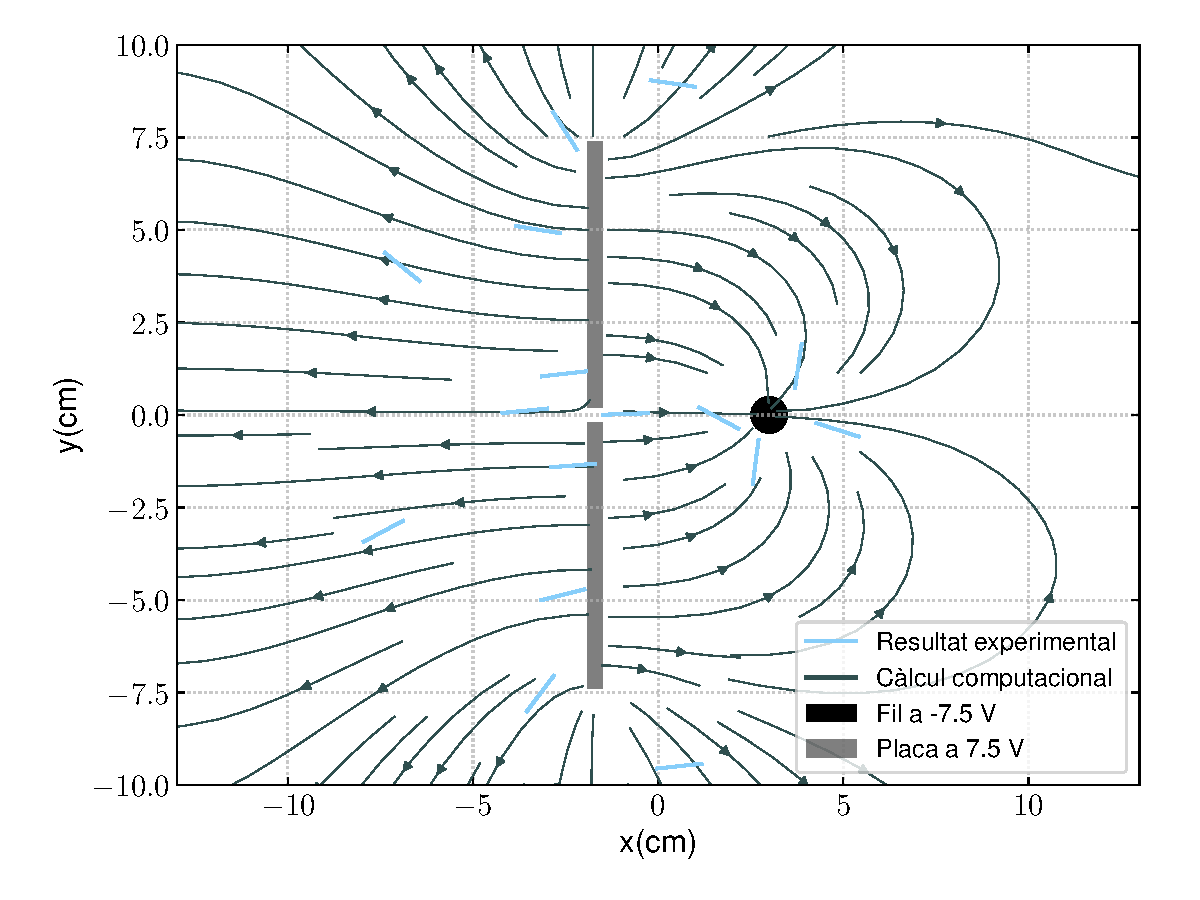
\includegraphics[width=0.45\textwidth]{lliure_camp.pdf}
    \caption{Línies de camp elèctric. Segments experimentals i línies de la simulació.}
    \label{fig: lliure_camp}
\end{figure}

Per altra banda, a la Fig. (\ref{fig: lliure_camp}) podem veure el camp elèctric generat per aquesta configuració. Com en les altres configuracions veiem que el camp experimental seguexi la tendència de la simulació però es tanca més al voltant de les vores de les plaques i dels fils infinits. Aquestes diferències s'expliquen pels mateixos raonaments que en els casos anteriors.


\subsection{(extra) Estimació de la permitivitat relativa}
A la Secció \ref{sec: cond} hem vist com les línies equipotencials simulades diferien de les experimentals principalment a causa de que la simulació està feta al buit, i en canvi, l'experiment emula un dielèctric. Aprofitarem aquestes diferencies per estimar el valor de la permitivitat relativa d'aquest dielèctric, $\varepsilon_r$.

En el cas ideal, dins del conductor, el camp elèctric queda fixat per la distància entre plaques, $d$, i la diferència de potencial $V$. Fora del condensador, però, el camp sí que depèn d'$\varepsilon_r$. 
Assumint que podem expressar el potencial al buit com 
\begin{equation}
    \phi_0 = \frac{U}{\varepsilon_0},
\end{equation} 
on $U$ és una funció desconeguda,\footnote{Això sempre ho podem fer perquè podem expressar el nostre sistema com la suma de moltes càrregues puntuals.} llavors el potencial en el dielèctric (l.i.h.) serà
\begin{equation}
    \phi(r)=\frac{\phi_0(r)}{\varepsilon_r}.
    \label{eq: epsilon}
\end{equation} 
Per poder treballar còmodament posem el zero de potencial a una de les dues plaques i per calcular $\varepsilon_r$ només hem d'evaluar l'Eq. (\ref{eq: epsilon}) a diferents punts. Concretament, agafem els punts experimentals del potencial i els substituïm per $\phi(r)$ i en els mateixos punts evaluem el potencial simulat al buit i el substituïm per $\phi_0(r)$. Així, obtenim el valor de $\varepsilon_r$ per cada parella de potencials en un mateix punt. Fent la mitjana entre els valors obtinguts hem estimat\footnote{Càlcul d'incerteses a l'Annex.}
\begin{equation}
    \varepsilon_r=(1,98 \pm 0,10)\, \mathrm{F/m}.
\end{equation}

\section{Conclusions}\label{sec: conc}

En aquesta pràctica hem estudiat les línies equipotencials i de camp dins d'un material dielèctric de tres configuracions de conductors diferents, gràcies al paral·lelisme entre les equacions del camp de corrents i del camp de desplaçament. 

En primer lloc hem estudiat un condensador de plaques plano-paral·leles finites només en una dimensió i hem pogut veure com, a diferència del cas ideal, les línies de camp es tanquen al voltant de les plaques. També hem vist com la simulació al buit coincideix en tendència amb l'experiment però les línies equipotencials simulades es tanquen més aprop de les plaques a causa de que el camp elèctric al buit és més intens que en el dielèctirc. A més, hem realitzat un càlcul experimental de la capacitat del condensador i hem obtingut un valor de $ \frac{C}{L} = \varepsilon  (2{,}51 \pm 0{,}63)\, \mathrm{F/m} $ que es compatible amb el resultat del model ideal.

En segon lloc hem estudiat dos fils infinits paral·lels a potencials oposats. En aquest cas hem pogut observar com les limitacions del nostre experiment per reproduïr aquesta configuració han provocat que les línies equipotencials fòssin el·líptiques en comptes de circulars.

En tercer lloc, hem estudiat una placa amb una escletxa davant d'un fil infinit a un potencial diferent amb l'objectiu de veure si les línies equipotencials pateixen algun fenòmen similar a la difracció d'una ona a causa de l'escletxa. Tanmateix, amb l'experiment hem constatat que no obstant les línies experimentals semblaven patir quelcom semblant a la difracció, amb la simulació hem pogut comprovar que la forma de les línies equipotencials quasi no depenia de si hi havia escletxa o no, i per tant, hem descartat aquesta idea.

Per últim, combinant els resultat experimentals i els de la simulació hem ideat una manera d'estimar el valor de la permitivitat relativa del medi dielèctric de l'experiment. Així hem obtingut un valor de $\varepsilon_r=(1,98 \pm 0,10)\, \mathrm{F/m}$.

\appendix{Annex}\label{sec: annex}
\section{Imatges del muntatge experimental}\label{fotos}
\begin{figure}[h!]
    \centering

    \begin{subcaptionbox}{Condensador\label{fig:img1}}[0.3\textwidth]
        {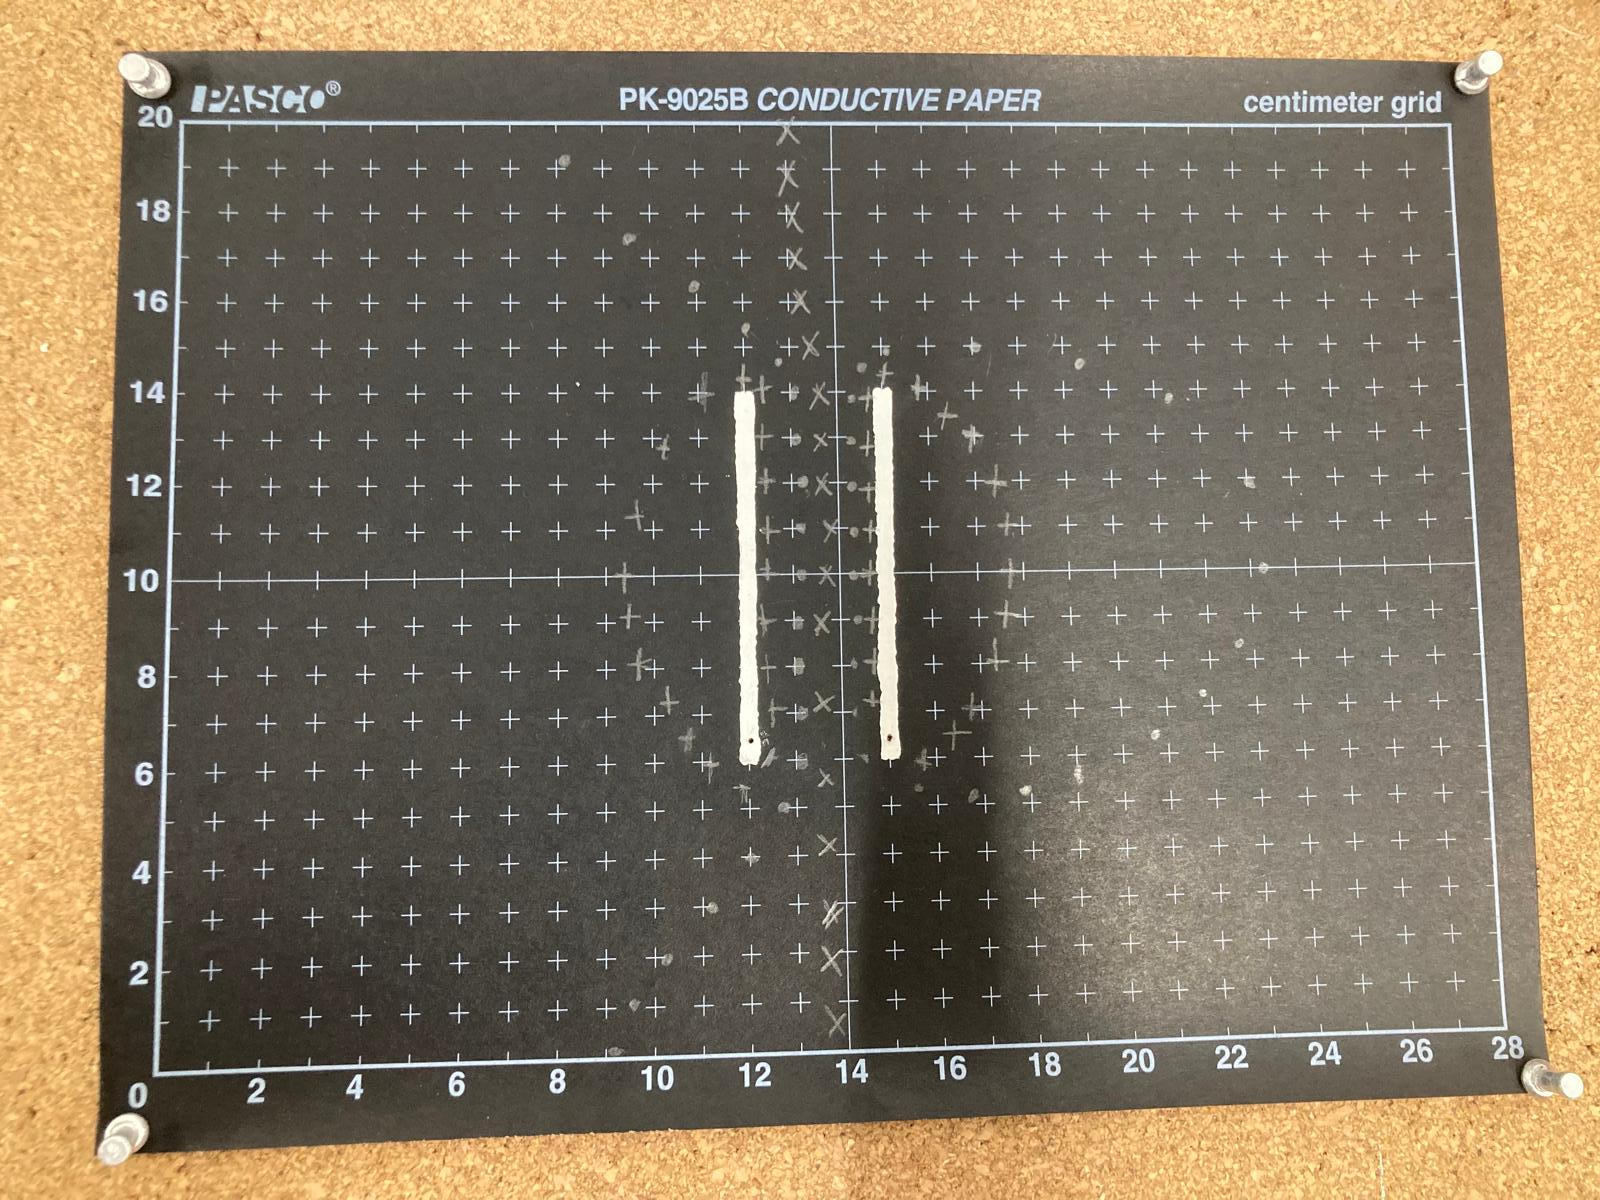
\includegraphics[width=\linewidth]{imatge1.jpg}}
    \end{subcaptionbox}
    \hfill
    \begin{subcaptionbox}{Fils inifnits\label{fig:img2}}[0.3\textwidth]
        {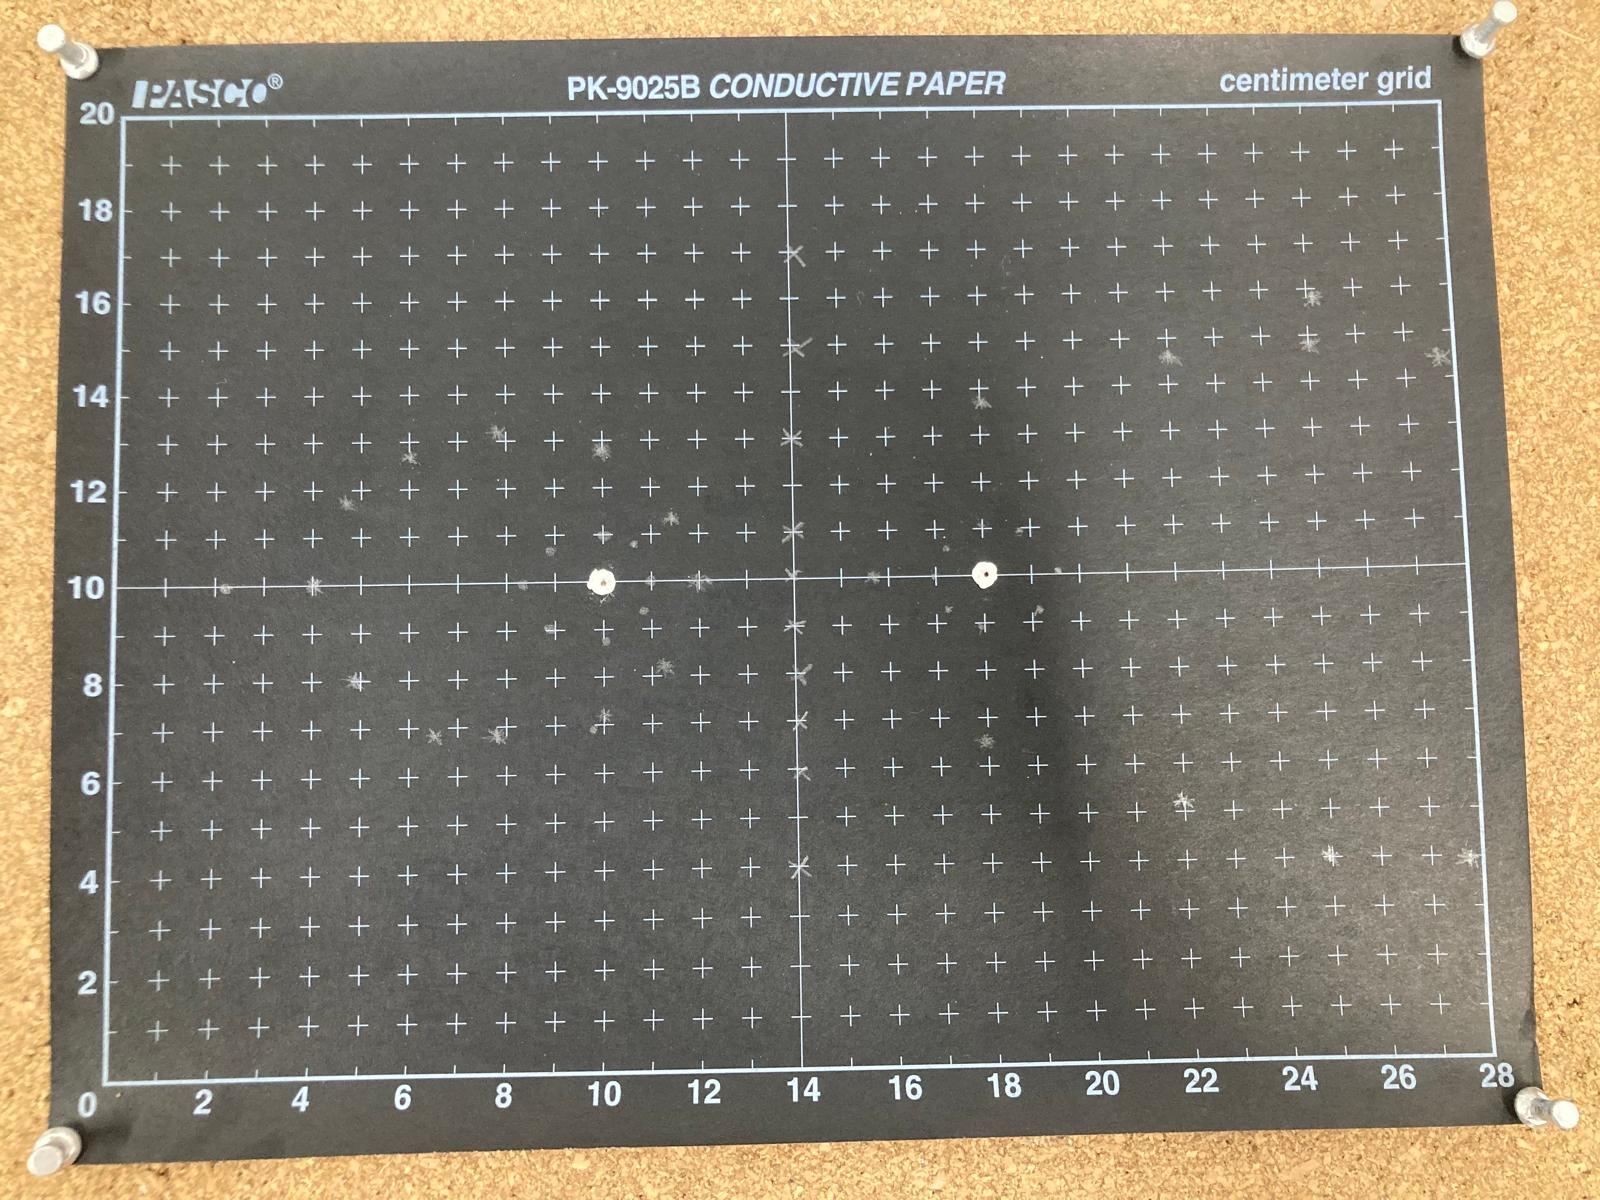
\includegraphics[width=\linewidth]{imatge2.jpg}}
    \end{subcaptionbox}
    \hfill
    \begin{subcaptionbox}{Configuració lliure\label{fig:img3}}[0.3\textwidth]
        {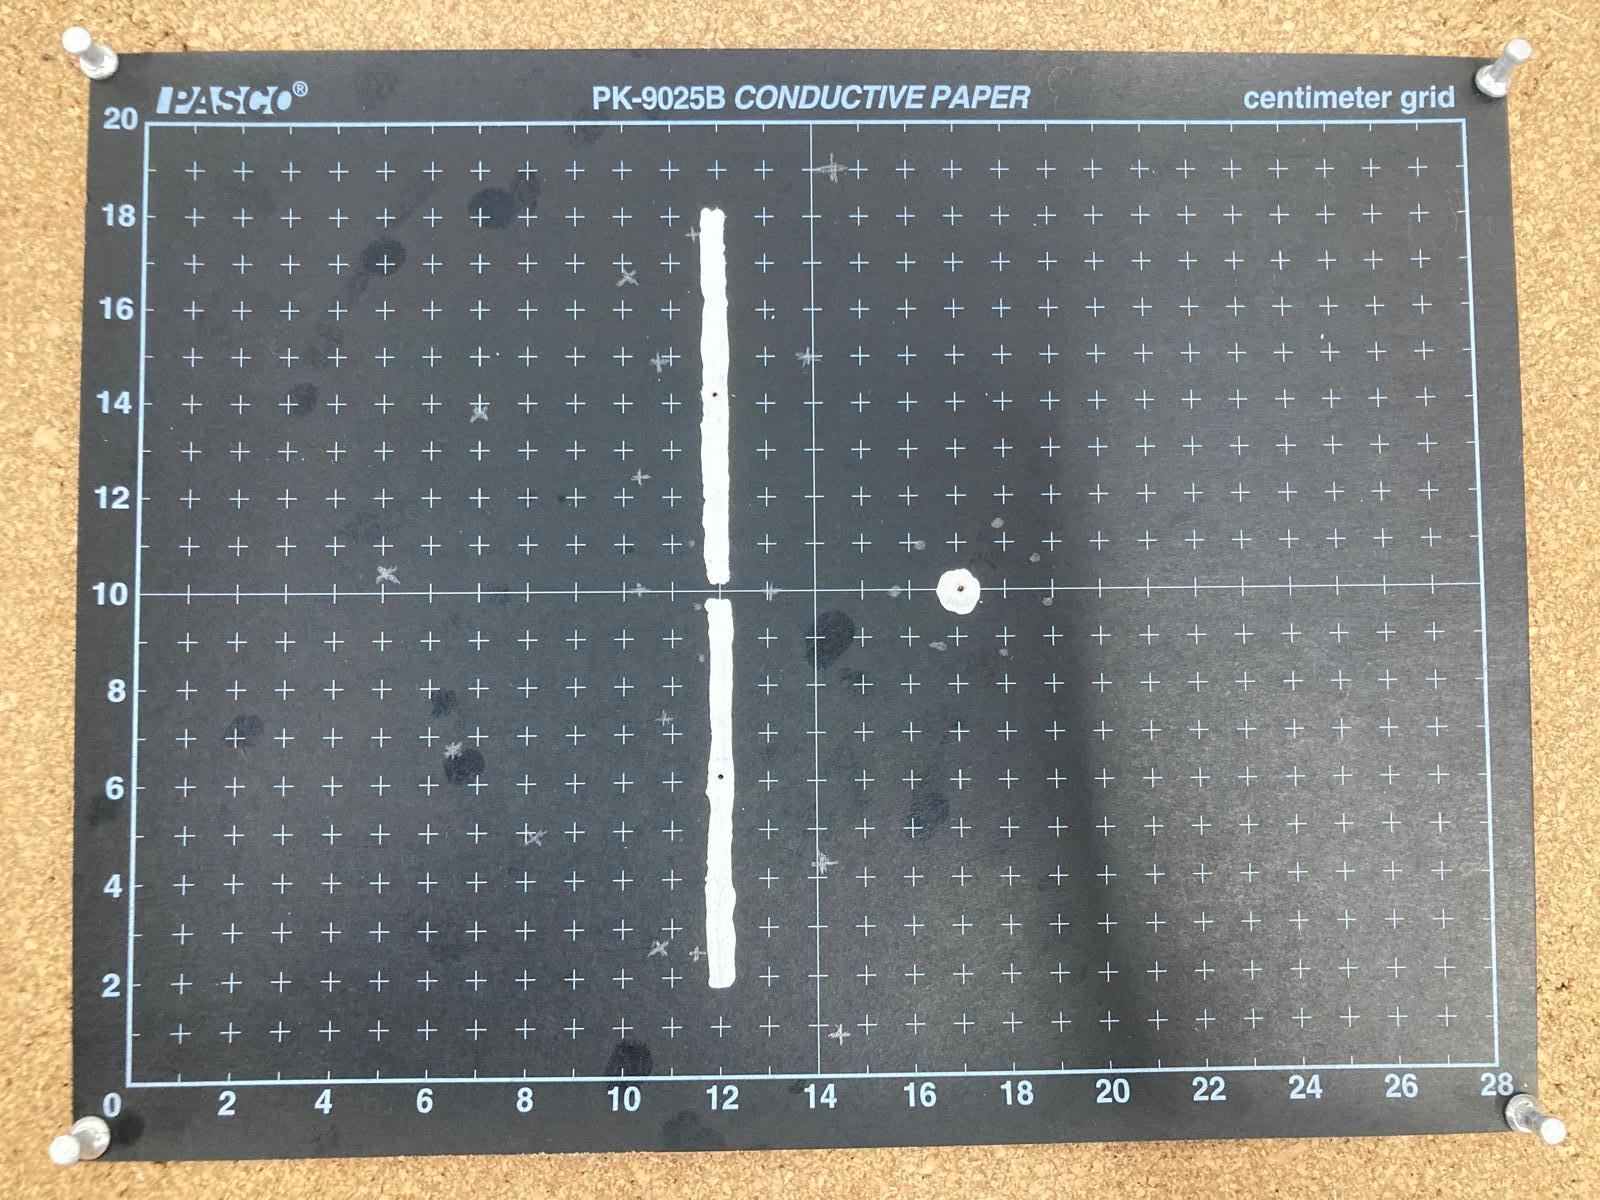
\includegraphics[width=\linewidth]{imatge3.jpg}}
    \end{subcaptionbox}

    \caption{Muntatge experimental de les tres distribucions de conductors.}
    \label{fig:figura3}
\end{figure}
\section{Càlcul d'incerteses}
\begin{equation}
    u_{Q/L} = \varepsilon \sqrt{
        \left( \sum_i \frac{\Delta l_i}{\Delta r_i} \right)^2 u^2_{\Delta \phi_i} +
        \left( \sum_i \frac{\Delta \phi_i}{\Delta r_i} \right)^2 u^2_{\Delta l_i} +
        \left( \sum_i \frac{\Delta \phi_i \Delta l_i}{\Delta r_i^2} \right)^2 u^2_{\Delta r_i}}
        \label{eq: ins_q}
\end{equation}


\begin{equation}
    u_{C/L} = \sqrt{
        \left( \frac{1}{\Delta V} \right)^2 u^2_{Q/L} +
        \left( \frac{Q/L}{\Delta V^2} \right)^2 u^2_{\Delta V}}
    \label{eq: ins_c}
\end{equation}

\begin{equation}
    u_{(C/L)_t} = \varepsilon \sqrt{
    \left( \frac{1}{d} \right)^2 u^2_l +
    \left( \frac{l}{d^2} \right)^2 u^2_d}
    \label{eq: ins_ct}
\end{equation}

\section{Dades experimentals}
\begin{table}[ht]
    \centering
    \begin{tabular}{ccc}
        \hline
        $\Delta l$ (m) & $\Delta r$ (m) & $\Delta V$ (V) \\
        \hline
        $0.009 \pm 0.001$ & $0.012 \pm 0.001$ & $1.5 \pm 0.1$ \\
        $0.007 \pm 0.001$ & $0.026 \pm 0.001$ & $1.5 \pm 0.1$ \\
        $0.011 \pm 0.001$ & $0.036 \pm 0.001$ & $1.5 \pm 0.1$ \\
        $0.011 \pm 0.001$ & $0.047 \pm 0.001$ & $1.5 \pm 0.1$ \\
        $0.009 \pm 0.001$ & $0.054 \pm 0.001$ & $1.5 \pm 0.1$ \\
        $0.001 \pm 0.001$ & $0.055 \pm 0.001$ & $1.5 \pm 0.1$ \\
        $0.009 \pm 0.001$ & $0.043 \pm 0.001$ & $1.5 \pm 0.1$ \\
        $0.011 \pm 0.001$ & $0.030 \pm 0.001$ & $1.5 \pm 0.1$ \\
        $0.006 \pm 0.001$ & $0.019 \pm 0.001$ & $1.5 \pm 0.1$ \\
        $0.008 \pm 0.001$ & $0.015 \pm 0.001$ & $1.5 \pm 0.1$ \\
        $0.007 \pm 0.001$ & $0.007 \pm 0.001$ & $1.5 \pm 0.1$ \\
        $0.005 \pm 0.001$ & $0.005 \pm 0.001$ & $1.5 \pm 0.1$ \\
        $0.010 \pm 0.001$ & $0.003 \pm 0.001$ & $1.5 \pm 0.1$ \\
        $0.010 \pm 0.001$ & $0.005 \pm 0.001$ & $1.5 \pm 0.1$ \\
        $0.009 \pm 0.001$ & $0.004 \pm 0.001$ & $1.5 \pm 0.1$ \\
        $0.010 \pm 0.001$ & $0.004 \pm 0.001$ & $1.5 \pm 0.1$ \\
        $0.010 \pm 0.001$ & $0.004 \pm 0.001$ & $1.5 \pm 0.1$ \\
        $0.010 \pm 0.001$ & $0.005 \pm 0.001$ & $1.5 \pm 0.1$ \\
        $0.008 \pm 0.001$ & $0.005 \pm 0.001$ & $1.5 \pm 0.1$ \\
        $0.015 \pm 0.001$ & $0.004 \pm 0.001$ & $1.5 \pm 0.1$ \\
        \hline
    \end{tabular}
    \caption{Mesures de $\Delta l$, $\Delta r$ i $\Delta V$ amb inserteses}
    \label{tab:mesures}
\end{table}

\section{Fitxers de programa de la simulació}\label{sec: python}
Per fer les simulacions de les línies equipotencials de les diferents configuracions de conductors hem solucionat l'equació de Laplace amb el mètode de Jacobi amb un programa de python. Aquí mostrem el probrama pel cas del condensador. Per calcular els altre casos només cal canviar les dimencions dels conductors ($l$ i $d$) i les condicions de contorn.

\begin{lstlisting}[caption={Simulació del potencial}, label={lst:simulacio}]
    import numpy as np
    import matplotlib.pyplot as plt

    # Dimensions de la malla
    nx, ny = 132, 132
    V = np.zeros((ny, nx))
    d = 15
    l = 40

    # Condicions de contorn (dos rectangles com plaques)
    V[int(ny/2-l/2):int(ny/2+l/2), int(nx/2 - d/2):int(nx/2 - d/2)+2] = 7.5  # placa esquerra
    V[int(ny/2-l/2):int(ny/2+l/2), int(nx/2 + d/2):int(nx/2 + d/2)+2] = -7.5    # placa dreta

    # Iteracio per resoldre Laplace (metode de Jacobi)
    for _ in range(6000):
        V_new = V.copy()
        V_new[1:-1,1:-1] = 0.25 * (V[1:-1, :-2] + V[1:-1, 2:] + V[:-2, 1:-1] + V[2:, 1:-1])
        
        # Reaplica condicions de contorn a la nova matriu
        V_new[int(ny/2-l/2):int(ny/2+l/2), int(nx/2 - d/2):int(nx/2 - d/2)+2] = 7.5
        V_new[int(ny/2-l/2):int(ny/2+l/2), int(nx/2 + d/2):int(nx/2 + d/2)+2] = -7.5
        
        V = V_new

    x = np.linspace(0, 27, nx)  # coordenades x
    y = np.linspace(0, 27, ny)  # coordenades y
    X, Y = np.meshgrid(x, y)
    ny, nx = V.shape

    # Aplanem les dades, les posem per columnes i canviem el centre de coordenades
    dades = np.column_stack((X.ravel()-13.5, Y.ravel()-13.5, V.ravel()))

    # Guardem com a txt: una fila = x y v
    np.savetxt("cond_teo_prova.txt", dades, fmt="%.6f", header="x y V", comments='')
\end{lstlisting}
Per trobar les línies de camp elèctric simulades hem calculat menys el gradient del potencial trobat anteriorment.
\begin{lstlisting}[caption={Simulació del camp elèctric}, label={lst:simulacio_camp}]
    import numpy as np
    import matplotlib.pyplot as plt
    Ey, Ex = np.gradient(-V)
    E = np.sqrt(Ex**2 + Ey**2)    
\end{lstlisting}

Per altra banda, per trobar les línies de camp elèctric experimentals hem calculat la direcció perpendicular a la recta entre dos punts adjacents de les línies equipotencials experimentals. Per fer-ho, hem creat dues funcions capaces de llegir un fitxer .txt amb les dades experimentals separades per valors de potencial mitjançant un espai en blanc i després calcular i representar segments amb la direcció del camp elèctric.

\begin{lstlisting}[caption={Camp elèctric experimental}, label={lst:exp_camp}]
    import numpy as np
    import matplotlib.pyplot as plt
    def llegir_equipotencials(filename):
    with open(filename, 'r') as f:
        contingut = f.read()

    blocs = contingut.strip().split('\n\n')
    llistes_coords = []

    for bloc in blocs:
        linies = bloc.strip().split('\n')
        coords = [list(map(float, linia.strip().split())) for linia in linies]
        llistes_coords.append(np.array(coords))

    return llistes_coords

    def representar_segments_llargs(equipotencials, salt=2, llargada=0.5):
        
        for coords in equipotencials:
            x = coords[:, 0]
            y = coords[:, 1]
            dx = np.gradient(x)
            dy = np.gradient(y)

            # Vector perpendicular
            Ex = -dy
            Ey = dx

            # Normalitzar
            mag = np.sqrt(Ex**2 + Ey**2)
            Ex_unit = Ex / mag
            Ey_unit = Ey / mag

            # Posicions i vectors reduits
            x_plot = x[::salt]
            y_plot = y[::salt]
            u = Ex_unit[::salt] * llargada / 2
            v = Ey_unit[::salt] * llargada / 2

            # Dibuixar segments (centrats)
            for xi, yi, ui, vi in zip(x_plot, y_plot, u, v):
                plt.plot([xi - ui, xi + ui], [yi - vi, yi + vi], color='lightskyblue')    
            plt.show()

    # === Executar ===
    fitxer = 'cond_exp.txt'
    equipotencials = llegir_equipotencials(fitxer)
    representar_segments_llargs(equipotencials, salt=2, llargada=1.2)
\end{lstlisting}
\end{document}
